\documentclass{article}


% if you need to pass options to natbib, use, e.g.:
%     \PassOptionsToPackage{numbers, compress}{natbib}
% before loading neurips_2024


% ready for submission
\usepackage{neurips_2024}


% to compile a preprint version, e.g., for submission to arXiv, add add the
% [preprint] option:
%     \usepackage[preprint]{neurips_2024}


% to compile a camera-ready version, add the [final] option, e.g.:
%     \usepackage[final]{neurips_2024}


% to avoid loading the natbib package, add option nonatbib:
%    \usepackage[nonatbib]{neurips_2024}


\usepackage[utf8]{inputenc} % allow utf-8 input
\usepackage[T1]{fontenc}    % use 8-bit T1 fonts
\usepackage{hyperref}       % hyperlinks
\usepackage{url}            % simple URL typesetting
\usepackage{booktabs}       % professional-quality tables
\usepackage{amsfonts}       % blackboard math symbols
\usepackage{nicefrac}       % compact symbols for 1/2, etc.
\usepackage{microtype}      % microtypography
\usepackage{xcolor}         % colors

% Packages added by me.
\usepackage{amsmath}
\usepackage{amssymb}
\usepackage{amsthm}
\usepackage{todonotes}
\usepackage{bm}
\usepackage{subcaption}
\usepackage[ruled]{algorithm2e}

\def\ci{\perp\!\!\!\!\!\perp}

\newtheorem{definition}{Definition}
\newtheorem{proposition}{Proposition}

\title{Title}


% The \author macro works with any number of authors. There are two commands
% used to separate the names and addresses of multiple authors: \And and \AND.
%
% Using \And between authors leaves it to LaTeX to determine where to break the
% lines. Using \AND forces a line break at that point. So, if LaTeX puts 3 of 4
% authors names on the first line, and the last on the second line, try using
% \AND instead of \And before the third author name.


\author{%
  David S.~Hippocampus\thanks{Use footnote for providing further information
    about author (webpage, alternative address)---\emph{not} for acknowledging
    funding agencies.} \\
  Department of Computer Science\\
  Cranberry-Lemon University\\
  Pittsburgh, PA 15213 \\
  \texttt{hippo@cs.cranberry-lemon.edu} \\
  % examples of more authors
  % \And
  % Coauthor \\
  % Affiliation \\
  % Address \\
  % \texttt{email} \\
  % \AND
  % Coauthor \\
  % Affiliation \\
  % Address \\
  % \texttt{email} \\
  % \And
  % Coauthor \\
  % Affiliation \\
  % Address \\
  % \texttt{email} \\
  % \And
  % Coauthor \\
  % Affiliation \\
  % Address \\
  % \texttt{email} \\
}

\begin{document}

\maketitle

\begin{abstract}
	\emph{Causal Discovery} involves learning causal structures
	from data, and has been studied both in Directed Acyclic Graphs
	(DAGs) and Structural Equation Models (SEMs). This problem has been
	extensively studied for both DAGs and SEMs. In the field of DAGs, many
	automated algorithms have been developed for constructing a DAG from a
	given dataset. However, the adaption of these algorithms in applied
	fields have been limited, possibly due to a lack of confidence in these
	algorithms stemming from them making obvious mistakes, and the
	difficulties in choosing the right algorithm for a given dataset.
	Consequently, in applied disciplines, these DAGs are predominantly
	constructed manually based on domain expertise. Due to being
	constructed by hand, it is vital that the fit of these models are
	tested against data and the models are potentially modified to acheive
	a better fit. On the other hand, in the field of SEMs models are
	typically constructed manually through an iterative process of
	assessing fit and modifying the model according to that. This process
	is commonly known as \emph{Specification Search} where methods like
	\emph{modification indices} can be used to guide this modification
	process. In the case of DAGs, although there are tests such as Shipley
	2000 that can assess the global fit of model by combining the tests
	using implied conditional independencies of the model, but there are no
	methods that can guide our modification process. In this paper, we
	present a simple modification process aimed at helping researchers in
	manually constructing or modifying the DAGs outputted by an algorithm.
	This modification process is based on using a measure of association
	for these individual local CI tests to identify the worst offending CI
	test and combining it with expert knowledge. We also present a measure
	of association based on canonical correlations for mixed data. We also
	present a graphical web-tool that can assist researchers in iteratively
	modifying and constructing their DAGs. We theoretically show that in
	the presence of an oracle, this iterative modification process is
	consistent in recovering the true DAG. Emprically, we show that this
	process performs comparably to PC and Hill-Climb Search algorithms if
	the user is able to correctly identify the direction of the edge in one
	out of three cases.
\end{abstract}

\section{Introduction}

To perform any causal effect identification or estimation in Pearl's Directed
Acyclic Graphs (DAGs) based causal framework usually requires to come up with
the DAG structure. Learning these DAG structures from data is known as
\emph{causal discovery}. Plenty of algorithms have been developed for these in
the literature such as constraint-based methods such as PC, FCI, score based
methods such as Hill-Climb Search, GES, and constrained continuous optimization
based such as No TEARS. All these algorithms take different approaches to
causal discovery, constraint-based algorithms utilize statistical conditional
independence (CI) tests to come up with a model structure, the score-based
methods iteratively perform local modifications to the model such that some
score function is maximized, the continuous optimization methods reformulate
the problem statement as a constrained optimization problem and use
optimization algorithms to come up with a graph.

Even though we have various algorithms for doing casual discovery, yet
researchers in applied fields prefer to construct these DAGs manually based on
their domain knowledge. We hypothesize the following two reasons for low
adaption of these methods in applied sciences:

\begin{enumerate}
	\item Biased towards sparse graphs.
	\item Algorithms making obvious mistakes: These algorithms often 
		make very obvious mistakes, making it harder for the user
		to trust them.
	\item Difficulties in choosing an algorithm: For any given dataset, the
		user need to make a choice of the algorithm. Given that these
		algorithms work very differently, it can be difficult to make a
		choice. Additionally, each of these algorithms have
		hyperparameters and choices to make for them, making it
		difficult. As there is no way to evaluate the performance of 
		these algorithms on our dataset.
\end{enumerate}
Both in the cases when the DAG is an output of an algorithm or when constructed
by hand, it is vital to test these models against data before using them for
making any inference. 

In the field of Structural Equation Models (SEMs), models are typically
constructed by hand. Researchers typically come up with an initial model, which
then they use the data to make modifications to. This process is known as
\emph{Specification Search}. One of the common ways to do this is through
\emph{modification indices} where a global fit of the model is measured with
different modification to the model. Utilizing expert knowledge to select the
appropriate modification that gives the maximum improvement to the global fit.

In the case of DAGs however, we do not have any way to 
As these CI based testing uses p-values and effect size measures from CI tests
for testing. And as mixed data is common, we need both a test and effect size
measure for mixed data. Recently, a few CI tests for mixed data have been
proposed but an effect size is still missing.

\begin{enumerate}
	\item We present a procedure to construct and modify DAGs using domain
		knowledge.
	\item The presented procedure uses a (conditional) measure of
		association between variables. In the simple case of continuous
		or discrete variables, effect size measures can be used,
		however as no such measure exists for mixed data, we present
		one.
	\item Lastly, to assist researchers in using the DAG construction
		approach, we developed a web-based tool to help researches in
		constructing and modifying their DAGs.
\end{enumerate}

\begin{figure}
		\centering
		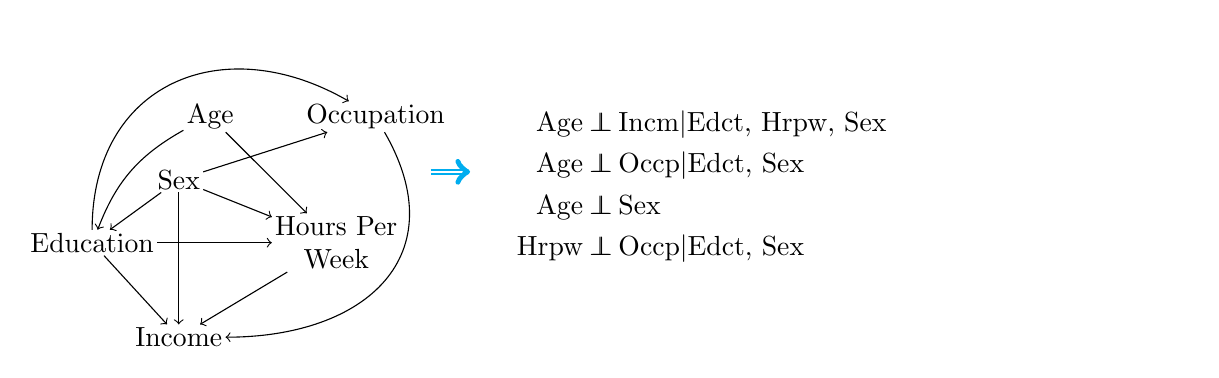
\begin{tikzpicture}
			\begin{scope}[yshift=0.7cm, scale=1]
			\tikzstyle{every node}=[align=center, inner sep=1pt]
				\node (sex) at (-0.7, -0.8) {Sex};
				\node (age) at (-0.3, 0) {Age};
				\node (ed) at (-1.8, -1.6) {Education};
				\node (occ) at (1.8, 0) {Occupation};
				\node (hrpw) at (1.3, -1.6) {Hours Per \\ Week};
				\node (income) at (-0.7, -2.8) {Income};
			
				\draw[->]  (age) to[bend right=20] (ed);
				\draw[->]  (sex) to (ed);
				\draw[->]  (age) to (hrpw);
				\draw[->]  (ed) to (hrpw);
				\draw[->]  (sex) to (hrpw);
				\draw[->]  (ed) to (income);
				\draw[->]  (hrpw) to (income);
				\draw[->]  (occ) to[out=300, in=0, looseness=1.4] (income.east);
				\draw[->]  (sex) to (income);
				\draw[->]  (ed) to[out=90, in=150, looseness=1.3] (occ);
				\draw[->]  (sex) to (occ);	
			\end{scope}
			\draw[thick, ->, double, cyan] (2.5,0) -- (3,0);
			\node[rectangle, align=center, inner sep=1pt] at (6, 0) {
				\begin{minipage}{\textwidth}
					\begin{equation*}
						\begin{split}
							\textnormal{Age} &\ci \textnormal{Incm} \rvert \textnormal{Edct, Hrpw, Sex} \\
							\textnormal{Age} &\ci \textnormal{Occp} \rvert \textnormal{Edct, Sex} \\
							\textnormal{Age} &\ci \textnormal{Sex} \\
							\textnormal{Hrpw} &\ci \textnormal{Occp} \rvert \textnormal{Edct, Sex} \\
						\end{split}
					\end{equation*}
				\end{minipage}
				};
		\end{tikzpicture}
		\caption{\todo[inline]{Show a full example of testing using this model}}
\end{figure}


\section{Background}
We represent uni-dimensional variables as $ X $ and multi-dimensional variables
as $ \bm{Z} $. We consider the case of estimating association between $ X $,
and $ Y $ is the presence of a set of conditioning variables $ \bm{Z} = Z_1,
\cdots, Z_k $, potentially being an empty set $ \bm{Z} = \emptyset $. We use $
\rvert \bm{Z} \rvert $ to denote the cardinality of the variable $ \bm{Z} $. We
consider various scenarios where the variables $ X $, $ Y $ and $ \bm{Z} $
could be either discrete, ordinal, or continuous. With mixed data, we mean an
arbitrary mix of variable types among $ X $, $ Y $, and $ \bm{Z} $.

We consider the problem of estimating the partial (or conditional) association
between $ X $ and $ Y $ in the presence of the conditioning set $ Z $. When $ Z
= \emptyset $, this is equivalent to the marginal association between $ X $ and
$ Y $.

\todo[inline]{Add more notation as they come}

\subsection{Effect size Measures}
In this section, we give a background on some of the commonly used effect size
measures in the context of CI testing.

\paragraph{$ X $ and $ Y $ are continuous}
In the case when $ \bm{Z} = \emptyset $, and when both $ X $ and $ Y $ are
continuous variables, Pearson's correlation coefficient based test can be used
which also gives an effect size measure. The p-value computation requires the
data to be normally distributed but other statistics can be used such as
Spearman's rank correlation, or Kendall's Tau.

In the case when $ \bm{Z} \neq \emptyset $, then partial correlations can be used.
In this case we first compute the residuals of $ X $ and $ Y $ using $ \bm{Z} $ as 
the predictor. We start by training two model $ X \sim \bm{Z} $ and $ Y \sim \bm{Z} $.
Then the residuals are computed for both as $ R_X = X - \hat{X} $ and $ R_Y = Y - \hat{Y} $.
After this we can do a normal non-conditional test on $ R_X $ and $ R_Y $.

\paragraph{All variables are discrete}

When $ \bm{Z} = \emptyset $, in the case of discrete variables, chi-squared test can be used. Effect size 
measures such as Cram\'er's V are available for it.

When $ \bm{Z} \neq \emptyset $, we can do stratification.


\paragraph{$ X $ is ordinal and $ Y $ is continuous}
Polyserial Correlation

When $ \bm{Z} = \emptyset $, ordinal variable can be assumed to be coming from a thresholded normal distribution, estimate the thresholds and latent variable to compute 
the correlation coefficient.

\paragraph{$ X $ and $ Y $ are ordinal}
Polychoric Correlation

\paragraph{Mixed data}
Recently multiple tests for mixed data have been proposed but they do not have
an effect size measure. We propose one based on canonical correlations.

\subsection{Canonical Correlation}
Canonical correlations are generalization of correlations to multi-dimensional variables.

\begin{definition}
	Given two sets of random variables $ \bm{U} = (U_1, U_2, \cdots, U_p) $
	and $ \bm{V} = (V_1, V_2, \cdots, V_q) $, canonical correlation between
	them, $\rho(\bm{U}, \bm{V}) $ is defined as:
		
	\begin{equation}
		\rho(\bm{U}, \bm{V}) = \sup_{a, b} \frac{a^T \Sigma_{\bm{U}\bm{V}} b}{\sqrt{a^T \Sigma_{\bm{U}\bm{U}} a} \sqrt{b^T \Sigma_{\bm{V}\bm{V}} b}}
	\end{equation}

\end{definition}
	
	Canonical correlations try to find linear transformations $ a $ and $ b
	$ of $ \bm{U} $ and $ \bm{V} $ such that the correlations between the
	columns of $ a^T \bm{U} $ and $ b^T \bm{V} $ is maximized. The
	individual columns of $ a^T \bm{U} $ and $ b^T \bm{V} $ are
	independent. In the case when $ \rvert U \rvert = \rvert V \rvert = 1$,
	canonical correlations are equivalent to Pearson's correlation
	coefficient.

Multiple effect sizes measures based on canonical correlation are available.
\begin{itemize}
	\item Wilks' Lambda: $ \Lambda = \prod (1 - \phi_i^2) $
	\item Roy's Largest Root: $ \theta = \phi_{\max}^2 $
	\item Pillai's Trace: $ \tau = \sum \phi_i^2 $
\end{itemize}
We use Pillai's Trace in this paper. \todo[inline]{Why?}.

\section{Effect size for mixed data}
In this section, we use canonical correlations to define an effect size measure
for mixed data CI tests. Our approach is similar to the approach used for the
continuous variable case. 

\subsection{No conditional variables}
When we have no conditonal variables, we need to convert the variables into 

\subsection{Conditional Case}

\subsection{Connection to special cases}

\section{Web Tool}
As most of the DAGs in practice are built manually, we use our mixed data effect size measure to build a web-tool that aids researches in building DAGs.

% \begin{figure}
% 	\centering
% 	\begin{subfigure}{0.5\textwidth}
% 		\includegraphics[scale=0.25]{../../presentations/2024_05_das/2.png}
% 	\end{subfigure}%
% 	\begin{subfigure}{0.5\textwidth}
% 		\includegraphics[scale=0.25]{../../presentations/2024_05_das/5.png}
% 	\end{subfigure}
% 	\caption{Screenshots of the web-tool. \todo[inline]{Insert screenshots of the web-tool}}
% \end{figure}

\section{Empirical Analysis}
To compare how well does creating a graph manually based on effect sizes and
p-value compare to algorithmic approaches, we performed some empirical
analysis.

\subsection{Simulating an expert}
To simulate an expert building a model manually, we wrote a simple greedy simulation as shown in the Figure. The expert always starts with a graph with
no edges and chooses the pair of variables with the highest correlation between them. The expert based on some accuracy measure decides the direction
of the edge between these variables such that the new added edge does not create a cycle in the DAG.

\todo[inline]{Summarize this section and equation in an algorithm}
\todo[inline]{Show a consistency proof for this expert simulation}

\begin{equation}
	\begin{split}
		x &= \textnormal{rand}([0, 1]) \\
		O(\alpha) &= \begin{cases} 
			M \rightarrow Y, & \textnormal{if  } x <= \alpha \\
			\textnormal{rand}(M \rightarrow Y, M \leftarrow Y, None) & \textnormal{otherwise} \\
				\end{cases} \\
	\end{split}
\end{equation}

\begin{algorithm}
	\caption{Expert Simulation}
	\While{True}{
	   $ e \gets \textnormal{Effects}(G) > \textnormal{THRESHOLD} $\;
	   $ e \gets e - \textnormal{blacklist} $\;
	   \If {$ e = 0 $}{
		$ G \gets G - e $ \;
		$ \textnormal{blacklist} \gets \textnormal{blacklist} \cup e $\;
	   } \;
	   \If{$ \textnormal{len}(e) = 0$}{
		   $ \textnormal{return}(G) $\;
	   }
	   $ X, Y \gets \max_{X, Y} e $\;
	   $ dir \gets Expert(X, Y, \alpha) $\;
	   $ G \gets G \cup dir $\;
	}

\end{algorithm}

After adding each edge, we also check if the p-value of any existing edge shows independence. If that happens we remove that edge and blacklist that edge. 
Blacklisted edges are not suggested to the expert in future iterations. We repeat this till we have explained all the correlations in the dataset.

There is a possibility that this greedy expert gets stuck at incorrect graph structures as it does not do any backtracking to fix its earlier mistakes.


\subsection{Results}
\begin{figure}
	\begin{subfigure}{0.5\textwidth}
		\includegraphics{../code/plots/shd_ribbon.pdf}
	\end{subfigure}%
	\begin{subfigure}{0.5\textwidth}
		\includegraphics{../code/plots/sid_ribbon.pdf}
	\end{subfigure}
\end{figure}

\section{Conclusions}
\subsection{Using LLMs as experts}



\bibliographystyle{plain}
\bibliography{references.bib}

%%%%%%%%%%%%%%%%%%%%%%%%%%%%%%%%%%%%%%%%%%%%%%%%%%%%%%%%%%%%

\appendix

\section{Appendix / supplemental material}


Optionally include supplemental material (complete proofs, additional experiments and plots) in appendix.
All such materials \textbf{SHOULD be included in the main submission.}

%%%%%%%%%%%%%%%%%%%%%%%%%%%%%%%%%%%%%%%%%%%%%%%%%%%%%%%%%%%%

\section*{NeurIPS Paper Checklist}

%%% BEGIN INSTRUCTIONS %%%
The checklist is designed to encourage best practices for responsible machine learning research, addressing issues of reproducibility, transparency, research ethics, and societal impact. Do not remove the checklist: {\bf The papers not including the checklist will be desk rejected.} The checklist should follow the references and precede the (optional) supplemental material.  The checklist does NOT count towards the page
limit. 

Please read the checklist guidelines carefully for information on how to answer these questions. For each question in the checklist:
\begin{itemize}
    \item You should answer \answerYes{}, \answerNo{}, or \answerNA{}.
    \item \answerNA{} means either that the question is Not Applicable for that particular paper or the relevant information is Not Available.
    \item Please provide a short (1–2 sentence) justification right after your answer (even for NA). 
   % \item {\bf The papers not including the checklist will be desk rejected.}
\end{itemize}

{\bf The checklist answers are an integral part of your paper submission.} They are visible to the reviewers, area chairs, senior area chairs, and ethics reviewers. You will be asked to also include it (after eventual revisions) with the final version of your paper, and its final version will be published with the paper.

The reviewers of your paper will be asked to use the checklist as one of the factors in their evaluation. While "\answerYes{}" is generally preferable to "\answerNo{}", it is perfectly acceptable to answer "\answerNo{}" provided a proper justification is given (e.g., "error bars are not reported because it would be too computationally expensive" or "we were unable to find the license for the dataset we used"). In general, answering "\answerNo{}" or "\answerNA{}" is not grounds for rejection. While the questions are phrased in a binary way, we acknowledge that the true answer is often more nuanced, so please just use your best judgment and write a justification to elaborate. All supporting evidence can appear either in the main paper or the supplemental material, provided in appendix. If you answer \answerYes{} to a question, in the justification please point to the section(s) where related material for the question can be found.

IMPORTANT, please:
\begin{itemize}
    \item {\bf Delete this instruction block, but keep the section heading ``NeurIPS paper checklist"},
    \item  {\bf Keep the checklist subsection headings, questions/answers and guidelines below.}
    \item {\bf Do not modify the questions and only use the provided macros for your answers}.
\end{itemize} 
 

%%% END INSTRUCTIONS %%%


\begin{enumerate}

\item {\bf Claims}
    \item[] Question: Do the main claims made in the abstract and introduction accurately reflect the paper's contributions and scope?
    \item[] Answer: \answerTODO{} % Replace by \answerYes{}, \answerNo{}, or \answerNA{}.
    \item[] Justification: \justificationTODO{}
    \item[] Guidelines:
    \begin{itemize}
        \item The answer NA means that the abstract and introduction do not include the claims made in the paper.
        \item The abstract and/or introduction should clearly state the claims made, including the contributions made in the paper and important assumptions and limitations. A No or NA answer to this question will not be perceived well by the reviewers. 
        \item The claims made should match theoretical and experimental results, and reflect how much the results can be expected to generalize to other settings. 
        \item It is fine to include aspirational goals as motivation as long as it is clear that these goals are not attained by the paper. 
    \end{itemize}

\item {\bf Limitations}
    \item[] Question: Does the paper discuss the limitations of the work performed by the authors?
    \item[] Answer: \answerTODO{} % Replace by \answerYes{}, \answerNo{}, or \answerNA{}.
    \item[] Justification: \justificationTODO{}
    \item[] Guidelines:
    \begin{itemize}
        \item The answer NA means that the paper has no limitation while the answer No means that the paper has limitations, but those are not discussed in the paper. 
        \item The authors are encouraged to create a separate "Limitations" section in their paper.
        \item The paper should point out any strong assumptions and how robust the results are to violations of these assumptions (e.g., independence assumptions, noiseless settings, model well-specification, asymptotic approximations only holding locally). The authors should reflect on how these assumptions might be violated in practice and what the implications would be.
        \item The authors should reflect on the scope of the claims made, e.g., if the approach was only tested on a few datasets or with a few runs. In general, empirical results often depend on implicit assumptions, which should be articulated.
        \item The authors should reflect on the factors that influence the performance of the approach. For example, a facial recognition algorithm may perform poorly when image resolution is low or images are taken in low lighting. Or a speech-to-text system might not be used reliably to provide closed captions for online lectures because it fails to handle technical jargon.
        \item The authors should discuss the computational efficiency of the proposed algorithms and how they scale with dataset size.
        \item If applicable, the authors should discuss possible limitations of their approach to address problems of privacy and fairness.
        \item While the authors might fear that complete honesty about limitations might be used by reviewers as grounds for rejection, a worse outcome might be that reviewers discover limitations that aren't acknowledged in the paper. The authors should use their best judgment and recognize that individual actions in favor of transparency play an important role in developing norms that preserve the integrity of the community. Reviewers will be specifically instructed to not penalize honesty concerning limitations.
    \end{itemize}

\item {\bf Theory Assumptions and Proofs}
    \item[] Question: For each theoretical result, does the paper provide the full set of assumptions and a complete (and correct) proof?
    \item[] Answer: \answerTODO{} % Replace by \answerYes{}, \answerNo{}, or \answerNA{}.
    \item[] Justification: \justificationTODO{}
    \item[] Guidelines:
    \begin{itemize}
        \item The answer NA means that the paper does not include theoretical results. 
        \item All the theorems, formulas, and proofs in the paper should be numbered and cross-referenced.
        \item All assumptions should be clearly stated or referenced in the statement of any theorems.
        \item The proofs can either appear in the main paper or the supplemental material, but if they appear in the supplemental material, the authors are encouraged to provide a short proof sketch to provide intuition. 
        \item Inversely, any informal proof provided in the core of the paper should be complemented by formal proofs provided in appendix or supplemental material.
        \item Theorems and Lemmas that the proof relies upon should be properly referenced. 
    \end{itemize}

    \item {\bf Experimental Result Reproducibility}
    \item[] Question: Does the paper fully disclose all the information needed to reproduce the main experimental results of the paper to the extent that it affects the main claims and/or conclusions of the paper (regardless of whether the code and data are provided or not)?
    \item[] Answer: \answerTODO{} % Replace by \answerYes{}, \answerNo{}, or \answerNA{}.
    \item[] Justification: \justificationTODO{}
    \item[] Guidelines:
    \begin{itemize}
        \item The answer NA means that the paper does not include experiments.
        \item If the paper includes experiments, a No answer to this question will not be perceived well by the reviewers: Making the paper reproducible is important, regardless of whether the code and data are provided or not.
        \item If the contribution is a dataset and/or model, the authors should describe the steps taken to make their results reproducible or verifiable. 
        \item Depending on the contribution, reproducibility can be accomplished in various ways. For example, if the contribution is a novel architecture, describing the architecture fully might suffice, or if the contribution is a specific model and empirical evaluation, it may be necessary to either make it possible for others to replicate the model with the same dataset, or provide access to the model. In general. releasing code and data is often one good way to accomplish this, but reproducibility can also be provided via detailed instructions for how to replicate the results, access to a hosted model (e.g., in the case of a large language model), releasing of a model checkpoint, or other means that are appropriate to the research performed.
        \item While NeurIPS does not require releasing code, the conference does require all submissions to provide some reasonable avenue for reproducibility, which may depend on the nature of the contribution. For example
        \begin{enumerate}
            \item If the contribution is primarily a new algorithm, the paper should make it clear how to reproduce that algorithm.
            \item If the contribution is primarily a new model architecture, the paper should describe the architecture clearly and fully.
            \item If the contribution is a new model (e.g., a large language model), then there should either be a way to access this model for reproducing the results or a way to reproduce the model (e.g., with an open-source dataset or instructions for how to construct the dataset).
            \item We recognize that reproducibility may be tricky in some cases, in which case authors are welcome to describe the particular way they provide for reproducibility. In the case of closed-source models, it may be that access to the model is limited in some way (e.g., to registered users), but it should be possible for other researchers to have some path to reproducing or verifying the results.
        \end{enumerate}
    \end{itemize}


\item {\bf Open access to data and code}
    \item[] Question: Does the paper provide open access to the data and code, with sufficient instructions to faithfully reproduce the main experimental results, as described in supplemental material?
    \item[] Answer: \answerTODO{} % Replace by \answerYes{}, \answerNo{}, or \answerNA{}.
    \item[] Justification: \justificationTODO{}
    \item[] Guidelines:
    \begin{itemize}
        \item The answer NA means that paper does not include experiments requiring code.
        \item Please see the NeurIPS code and data submission guidelines (\url{https://nips.cc/public/guides/CodeSubmissionPolicy}) for more details.
        \item While we encourage the release of code and data, we understand that this might not be possible, so “No” is an acceptable answer. Papers cannot be rejected simply for not including code, unless this is central to the contribution (e.g., for a new open-source benchmark).
        \item The instructions should contain the exact command and environment needed to run to reproduce the results. See the NeurIPS code and data submission guidelines (\url{https://nips.cc/public/guides/CodeSubmissionPolicy}) for more details.
        \item The authors should provide instructions on data access and preparation, including how to access the raw data, preprocessed data, intermediate data, and generated data, etc.
        \item The authors should provide scripts to reproduce all experimental results for the new proposed method and baselines. If only a subset of experiments are reproducible, they should state which ones are omitted from the script and why.
        \item At submission time, to preserve anonymity, the authors should release anonymized versions (if applicable).
        \item Providing as much information as possible in supplemental material (appended to the paper) is recommended, but including URLs to data and code is permitted.
    \end{itemize}


\item {\bf Experimental Setting/Details}
    \item[] Question: Does the paper specify all the training and test details (e.g., data splits, hyperparameters, how they were chosen, type of optimizer, etc.) necessary to understand the results?
    \item[] Answer: \answerTODO{} % Replace by \answerYes{}, \answerNo{}, or \answerNA{}.
    \item[] Justification: \justificationTODO{}
    \item[] Guidelines:
    \begin{itemize}
        \item The answer NA means that the paper does not include experiments.
        \item The experimental setting should be presented in the core of the paper to a level of detail that is necessary to appreciate the results and make sense of them.
        \item The full details can be provided either with the code, in appendix, or as supplemental material.
    \end{itemize}

\item {\bf Experiment Statistical Significance}
    \item[] Question: Does the paper report error bars suitably and correctly defined or other appropriate information about the statistical significance of the experiments?
    \item[] Answer: \answerTODO{} % Replace by \answerYes{}, \answerNo{}, or \answerNA{}.
    \item[] Justification: \justificationTODO{}
    \item[] Guidelines:
    \begin{itemize}
        \item The answer NA means that the paper does not include experiments.
        \item The authors should answer "Yes" if the results are accompanied by error bars, confidence intervals, or statistical significance tests, at least for the experiments that support the main claims of the paper.
        \item The factors of variability that the error bars are capturing should be clearly stated (for example, train/test split, initialization, random drawing of some parameter, or overall run with given experimental conditions).
        \item The method for calculating the error bars should be explained (closed form formula, call to a library function, bootstrap, etc.)
        \item The assumptions made should be given (e.g., Normally distributed errors).
        \item It should be clear whether the error bar is the standard deviation or the standard error of the mean.
        \item It is OK to report 1-sigma error bars, but one should state it. The authors should preferably report a 2-sigma error bar than state that they have a 96\% CI, if the hypothesis of Normality of errors is not verified.
        \item For asymmetric distributions, the authors should be careful not to show in tables or figures symmetric error bars that would yield results that are out of range (e.g. negative error rates).
        \item If error bars are reported in tables or plots, The authors should explain in the text how they were calculated and reference the corresponding figures or tables in the text.
    \end{itemize}

\item {\bf Experiments Compute Resources}
    \item[] Question: For each experiment, does the paper provide sufficient information on the computer resources (type of compute workers, memory, time of execution) needed to reproduce the experiments?
    \item[] Answer: \answerTODO{} % Replace by \answerYes{}, \answerNo{}, or \answerNA{}.
    \item[] Justification: \justificationTODO{}
    \item[] Guidelines:
    \begin{itemize}
        \item The answer NA means that the paper does not include experiments.
        \item The paper should indicate the type of compute workers CPU or GPU, internal cluster, or cloud provider, including relevant memory and storage.
        \item The paper should provide the amount of compute required for each of the individual experimental runs as well as estimate the total compute. 
        \item The paper should disclose whether the full research project required more compute than the experiments reported in the paper (e.g., preliminary or failed experiments that didn't make it into the paper). 
    \end{itemize}
    
\item {\bf Code Of Ethics}
    \item[] Question: Does the research conducted in the paper conform, in every respect, with the NeurIPS Code of Ethics \url{https://neurips.cc/public/EthicsGuidelines}?
    \item[] Answer: \answerTODO{} % Replace by \answerYes{}, \answerNo{}, or \answerNA{}.
    \item[] Justification: \justificationTODO{}
    \item[] Guidelines:
    \begin{itemize}
        \item The answer NA means that the authors have not reviewed the NeurIPS Code of Ethics.
        \item If the authors answer No, they should explain the special circumstances that require a deviation from the Code of Ethics.
        \item The authors should make sure to preserve anonymity (e.g., if there is a special consideration due to laws or regulations in their jurisdiction).
    \end{itemize}


\item {\bf Broader Impacts}
    \item[] Question: Does the paper discuss both potential positive societal impacts and negative societal impacts of the work performed?
    \item[] Answer: \answerTODO{} % Replace by \answerYes{}, \answerNo{}, or \answerNA{}.
    \item[] Justification: \justificationTODO{}
    \item[] Guidelines:
    \begin{itemize}
        \item The answer NA means that there is no societal impact of the work performed.
        \item If the authors answer NA or No, they should explain why their work has no societal impact or why the paper does not address societal impact.
        \item Examples of negative societal impacts include potential malicious or unintended uses (e.g., disinformation, generating fake profiles, surveillance), fairness considerations (e.g., deployment of technologies that could make decisions that unfairly impact specific groups), privacy considerations, and security considerations.
        \item The conference expects that many papers will be foundational research and not tied to particular applications, let alone deployments. However, if there is a direct path to any negative applications, the authors should point it out. For example, it is legitimate to point out that an improvement in the quality of generative models could be used to generate deepfakes for disinformation. On the other hand, it is not needed to point out that a generic algorithm for optimizing neural networks could enable people to train models that generate Deepfakes faster.
        \item The authors should consider possible harms that could arise when the technology is being used as intended and functioning correctly, harms that could arise when the technology is being used as intended but gives incorrect results, and harms following from (intentional or unintentional) misuse of the technology.
        \item If there are negative societal impacts, the authors could also discuss possible mitigation strategies (e.g., gated release of models, providing defenses in addition to attacks, mechanisms for monitoring misuse, mechanisms to monitor how a system learns from feedback over time, improving the efficiency and accessibility of ML).
    \end{itemize}
    
\item {\bf Safeguards}
    \item[] Question: Does the paper describe safeguards that have been put in place for responsible release of data or models that have a high risk for misuse (e.g., pretrained language models, image generators, or scraped datasets)?
    \item[] Answer: \answerTODO{} % Replace by \answerYes{}, \answerNo{}, or \answerNA{}.
    \item[] Justification: \justificationTODO{}
    \item[] Guidelines:
    \begin{itemize}
        \item The answer NA means that the paper poses no such risks.
        \item Released models that have a high risk for misuse or dual-use should be released with necessary safeguards to allow for controlled use of the model, for example by requiring that users adhere to usage guidelines or restrictions to access the model or implementing safety filters. 
        \item Datasets that have been scraped from the Internet could pose safety risks. The authors should describe how they avoided releasing unsafe images.
        \item We recognize that providing effective safeguards is challenging, and many papers do not require this, but we encourage authors to take this into account and make a best faith effort.
    \end{itemize}

\item {\bf Licenses for existing assets}
    \item[] Question: Are the creators or original owners of assets (e.g., code, data, models), used in the paper, properly credited and are the license and terms of use explicitly mentioned and properly respected?
    \item[] Answer: \answerTODO{} % Replace by \answerYes{}, \answerNo{}, or \answerNA{}.
    \item[] Justification: \justificationTODO{}
    \item[] Guidelines:
    \begin{itemize}
        \item The answer NA means that the paper does not use existing assets.
        \item The authors should cite the original paper that produced the code package or dataset.
        \item The authors should state which version of the asset is used and, if possible, include a URL.
        \item The name of the license (e.g., CC-BY 4.0) should be included for each asset.
        \item For scraped data from a particular source (e.g., website), the copyright and terms of service of that source should be provided.
        \item If assets are released, the license, copyright information, and terms of use in the package should be provided. For popular datasets, \url{paperswithcode.com/datasets} has curated licenses for some datasets. Their licensing guide can help determine the license of a dataset.
        \item For existing datasets that are re-packaged, both the original license and the license of the derived asset (if it has changed) should be provided.
        \item If this information is not available online, the authors are encouraged to reach out to the asset's creators.
    \end{itemize}

\item {\bf New Assets}
    \item[] Question: Are new assets introduced in the paper well documented and is the documentation provided alongside the assets?
    \item[] Answer: \answerTODO{} % Replace by \answerYes{}, \answerNo{}, or \answerNA{}.
    \item[] Justification: \justificationTODO{}
    \item[] Guidelines:
    \begin{itemize}
        \item The answer NA means that the paper does not release new assets.
        \item Researchers should communicate the details of the dataset/code/model as part of their submissions via structured templates. This includes details about training, license, limitations, etc. 
        \item The paper should discuss whether and how consent was obtained from people whose asset is used.
        \item At submission time, remember to anonymize your assets (if applicable). You can either create an anonymized URL or include an anonymized zip file.
    \end{itemize}

\item {\bf Crowdsourcing and Research with Human Subjects}
    \item[] Question: For crowdsourcing experiments and research with human subjects, does the paper include the full text of instructions given to participants and screenshots, if applicable, as well as details about compensation (if any)? 
    \item[] Answer: \answerTODO{} % Replace by \answerYes{}, \answerNo{}, or \answerNA{}.
    \item[] Justification: \justificationTODO{}
    \item[] Guidelines:
    \begin{itemize}
        \item The answer NA means that the paper does not involve crowdsourcing nor research with human subjects.
        \item Including this information in the supplemental material is fine, but if the main contribution of the paper involves human subjects, then as much detail as possible should be included in the main paper. 
        \item According to the NeurIPS Code of Ethics, workers involved in data collection, curation, or other labor should be paid at least the minimum wage in the country of the data collector. 
    \end{itemize}

\item {\bf Institutional Review Board (IRB) Approvals or Equivalent for Research with Human Subjects}
    \item[] Question: Does the paper describe potential risks incurred by study participants, whether such risks were disclosed to the subjects, and whether Institutional Review Board (IRB) approvals (or an equivalent approval/review based on the requirements of your country or institution) were obtained?
    \item[] Answer: \answerTODO{} % Replace by \answerYes{}, \answerNo{}, or \answerNA{}.
    \item[] Justification: \justificationTODO{}
    \item[] Guidelines:
    \begin{itemize}
        \item The answer NA means that the paper does not involve crowdsourcing nor research with human subjects.
        \item Depending on the country in which research is conducted, IRB approval (or equivalent) may be required for any human subjects research. If you obtained IRB approval, you should clearly state this in the paper. 
        \item We recognize that the procedures for this may vary significantly between institutions and locations, and we expect authors to adhere to the NeurIPS Code of Ethics and the guidelines for their institution. 
        \item For initial submissions, do not include any information that would break anonymity (if applicable), such as the institution conducting the review.
    \end{itemize}

\end{enumerate}



\end{document}
